\documentclass[10pt]{article}

\usepackage[margin=0.75in]{geometry}
\usepackage{amsmath,amsthm,amssymb}
\usepackage{xcolor}
\usepackage{cancel}
\usepackage{graphicx}
\usepackage{changepage}
\usepackage{circuitikz}
\usepackage{pgfplots}
\usepackage{subcaption}
\usepackage{physics}
\usepackage{siunitx}
\usepackage{minted}
\usepackage{robust-externalize}
\usepackage[breakable]{tcolorbox}
\usepackage[inline]{enumitem}

\theoremstyle{definition}
\newtheorem{problem}{Problem}
\newtheorem{soln}{Solution}

\pgfplotsset{compat=newest}
\usetikzlibrary{lindenmayersystems}
\usetikzlibrary{arrows}
\robExtConfigure{enable fallback to manual mode} % prints command to run in PDF if shell-escape is not used/forgotten
\def\mathdefault#1{#1} % Needed in matplotlib 3.8: https://github.com/matplotlib/matplotlib/issues/27907

\definecolor{incolor}{HTML}{303F9F}
\definecolor{outcolor}{HTML}{D84315}
\definecolor{cellborder}{HTML}{CFCFCF}
\definecolor{cellbackground}{HTML}{F7F7F7}
\newcommand{\eq}{=}
\tikzset
{%
  axes/.style={thick,-latex},
  cylinder/.style={right color=blue!80,left color=white,fill opacity=0.7},
  paraboloid back/.style={left color=magenta!80,fill opacity=0.4},
  paraboloid front/.style={left color=white, right color=magenta!80,fill opacity=0.4},
}       

\makeatletter
\newcommand{\boxspacing}{\kern\kvtcb@left@rule\kern\kvtcb@boxsep}
\makeatother
\newcommand{\prompt}[4]{
    \ttfamily\llap{{\color{#2}[#3]:\hspace{3pt}#4}}\vspace{-\baselineskip}
}

\newcommand{\highlight}[1]{\colorbox{yellow}{$\displaystyle #1$}}

\NewDocumentCommand{\evalat}{sO{\big}mm}{%
  \IfBooleanTF{#1}
   {\mleft. #3 \mright|_{#4}}
   {#3#2|_{#4}}%
}

\begin{PlaceholderFromCode}{__MY_MATPLOTLIB_START__}
      import matplotlib.pyplot as plt
      import matplotlib
      from matplotlib.pyplot import figure
      matplotlib.use("pgf")
      # https://matplotlib.org/stable/users/explain/text/pgf.html
      matplotlib.rcParams.update({
        "font.family": "serif",
        "font.serif": [], # Use LaTeX default serif font.
        "text.usetex": True, # use inline math for ticks
        ## You can change the font size of individual items with:
        # "font.size": 11,
        # "axes.titlesize": 11,
        # "legend.fontsize": 11,
        # "axes.labelsize": 11,
      })
      figure(figsize=(__MY_MATPLOTLIB_WIDTH__, __MY_MATPLOTLIB_HEIGHT__))
      \end{PlaceholderFromCode}
      
      \begin{PlaceholderFromCode}{__MY_MATPLOTLIB_END__}
      # https://stackoverflow.com/a/52587591/4987648
      plt.savefig(get_filename_from_extension(".pgf"), bbox_inches="tight")
      \end{PlaceholderFromCode}
      
      \robExtConfigure{
        new preset={my matplotlib pgf}{
          python,
          % If you want to include it via a simple input
          custom include command={\input{\robExtAddCachePathAndName{\robExtFinalHash.pgf}}},
          % If you also want to cache the tikz code for faster rendering
          % (otherwise only python -> tikz will be cached, but not tikz -> pdf)
          % custom include command={\evalPlaceholder{\cacheMe[tikz]{\input{__ROBEXT_OUTPUT_PREFIX__.pgf}}}},
          set placeholder eval={__LINEWIDTH__}{\lenToCmNoUnit[in]{\linewidth}},
          add import={__MY_MATPLOTLIB_START__},
          add to placeholder={__ROBEXT_MAIN_CONTENT__}{__MY_MATPLOTLIB_END__},
          %% Create a few functions to change the width easily:
          set size inches/.style 2 args={
            set placeholder={__MY_MATPLOTLIB_WIDTH__}{#1},
            set placeholder={__MY_MATPLOTLIB_HEIGHT__}{#2},
          },
          set size cm/.style 2 args={
            set size inches={#1/2.54}{#2/2.54},
          },
          set size pc/.style 2 args={
            set size inches={#1*__LINEWIDTH__}{#2*__LINEWIDTH__},
          },
          set size pc={1}{.7}, % default size
        }
      }

\title{Physics 2130: Assignment III}
\author{Jeremy Favro}
\date{\today}

\begin{document}

\maketitle

% PROBLEM 1
\begin{problem}
Consider the driven, damped harmonic oscillator. Its equation of motion is:
$$\ddot{x}+2\beta\dot{x}+\omega_0^2=A\cos\left(\omega t\right)$$
In the case of an underdamped oscillator, i.e., $\beta<\omega_0^2$ we found that the solution for the equation of motion is:
$$x(t)=x_c(t)+x_p(t)$$
Where:
$$x_c(t)e^{-\beta t}\left[c_1e^{i\omega_1 t}+c_2e^{-i\omega_1 t}\right]=Be^{-\beta t}\cos\left(\omega_1 t-\phi\right)=\Gamma(t)s(t)$$
And where:
$$\omega_1=\sqrt{w_0^2-\beta^2}$$
$$\Gamma(t)=Be^{-\beta t}$$
$$s(t)=\cos\left(\omega_1 t-\phi\right)$$
The particular solution is instead:
$$x_p(t)=D\cos\left(\omega t-\delta\right)$$
Where:
$$D=\frac{A}{\sqrt{\left(\omega_0^2-\omega^2\right)^2+4\omega^2\beta^2}}$$
$$\delta=\arctan\left(\frac{2\omega\beta}{\omega_0^2-\omega^2}\right)$$
\begin{enumerate}[label=(\alph*)]
      \item Consider an underdamped driven oscillator that starts with the initial conditions $x(t=0)=x_0$ and $\dot{x}(t=0)=0$.
            Find the analytical expressions for the unknown coefficients in $x(t)$ using these initial conditions.

      \item Write a python program that returns (and prints) the values of $\omega_1$, $\beta$, $\phi$, $D$ and $\delta$ for a given $x_0$. This should
            be coded as a function called \verb|harm_osc_params| that accepts as inputs $\omega_0$, $\beta$, $A$, $\omega$ and $x_0$.

      \item In the same python program, now write a new function, \verb|harm_osc_x_pos|, that calculates the array of positions $x$ of the
            harmonic oscillator for a given array of times $t$. This function should receive the array $t$ as an input as well as the values of $\omega_0$,
            $\beta$, $A$, $\omega$ and $x_0$. It should call the previously written function \verb|harm_osc_params| for the calculations of all the oscillation parameters.
            It should return the array of positions $x$ of the harmonic oscillator for each value of $t$.

      \item In the same python program, now write a new function to plot the data, \verb|harm_osc_x_plot_single|. The
            function receives as inputs the arrays $t$ and $x$ generated at the previous step.

      \item Pick three values of $\beta$ (remember of the constraint $\beta<w_0$) and plot in the same graph $x(t)$ for the three
            chosen values. For reference use $w_0=1\unit{\per\second}$ and $A=1\unit{\per\second\squared}$ (but play with the values of $A$ to see the relative
            importance of the driver and the damping). Comment on what effect $\beta$ has on both the transient and steady-state solution.

      \item To help you distinguish the different effects, now write a function called \verb|harm_osc_damp_drive| that plots
            in the same graph, $s(t)$, $\Gamma(t)$, $x_c(t)$ and $x_p(t)$. Comment on the results, specifically on the contribution of each component.

      \item Finally, write a new function called \verb|harm_osc_euler_cromer| that receives has input parameters $\omega_0$, $\beta$,
            $A$, $\omega$, $x_0$, and the analytical solution $x(t)$. This function should calculate a new $x(t)$, called $x_{EC}(t)$, that uses
            the Euler-Cromer method to determine the position of the oscillator as a function of time for the same initial conditions. Additionally, the function should
            plot, on the same graph, the solutions $x(t)$ and $x_{EC}(t)$ obtained with the analytical and Euler-Cromer methods, respectively, and the residuals, i.e.,
            the difference $x(t)-x_{EC}(t)$. Discuss how you choose a value of $\Delta t$ that gives a sufficiently accurate answer (which means defining
            ``sufficiently accurate'').
\end{enumerate}
\end{problem}
\begin{soln}~
      \begin{enumerate}[label=(\alph*)]
            \item \begin{align*}
                         & x(t=0)=B\cos\left(-\phi\right)+D\cos\left(-\delta\right)=x_0             \\
                         & \Rightarrow x_0-D\cos\left(\delta\right)=B\cos\left(\phi\right)          \\
                         & \Rightarrow \frac{x_0-D\cos\left(\delta\right)}{\cos\left(\phi\right)}=B \\
                  \end{align*}
                  \begin{align*}
                         & \dot{x}(t=0)=-B\omega_1\sin\left(-\phi\right)-B\beta\cos\left(-\phi\right)-D\omega\sin\left(-\delta\right)=0                                                                                                 \\
                         & =B\omega_1\sin\left(\phi\right)-B\beta\cos\left(\phi\right)+D\omega\sin\left(\delta\right)                                                                                                                   \\
                         & =\frac{x_0-D\cos\left(\delta\right)}{\cos\left(\phi\right)}\omega_1\sin\left(\phi\right)-\frac{x_0-D\cos\left(\delta\right)}{\cos\left(\phi\right)}\beta\cos\left(\phi\right)+D\omega\sin\left(\delta\right) \\
                         & =\left(x_0-D\cos\left(\delta\right)\right)\omega_1\tan\left(\phi\right)-\left(x_0-D\cos\left(\delta\right)\right)\beta+D\omega\sin\left(\delta\right)                                                        \\
                         & \Rightarrow -\frac{D\omega\sin\left(\delta\right)}{\left(x_0-D\cos\left(\delta\right)\right)}=\omega_1\tan\left(\phi\right)-\beta                                                                            \\
                         & \Rightarrow \arctan\left(\frac{\beta-\frac{D\omega\sin\left(\delta\right)}{\left(x_0-D\cos\left(\delta\right)\right)}}{\omega_1}\right)=\phi                                                                 \\
                  \end{align*}

            \item \inputminted[breaklines, autogobble]{python3}{./python/q1/q1b.py} % TODO: Figure out imports or something idk.
                  \newpage
            \item \inputminted[breaklines, autogobble]{python3}{./python/q1/q1c.py}

            \item \inputminted[breaklines, autogobble]{python3}{./python/q1/q1d.py}
                  \begin{center}
                        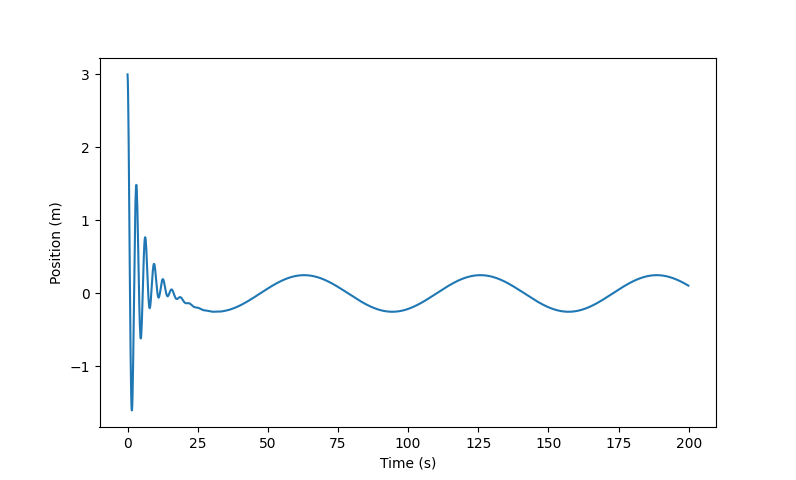
\includegraphics[scale=0.75]{Figure_1.png}
                  \end{center}
                  The first regime, visible as the rapid oscillations from $t=0$ to $t\approx 30$ is dominated by the $Be^{-\beta t}\cos\left(\omega_1 t-\phi\right)$ term. Because
                  This term contains an exponential decay factor it will fade away as time progresses leaving the $D\cos\left(\omega t-\delta\right)$ term as the only oscillator.
                  The first regime has a period of $\approx 3.2\unit{\radian\per\second}$, which is consistent with $\omega_1=\frac{2\pi}{\sqrt{w_0^2-\beta^2}}=\frac{2\pi}{\sqrt{2^2-0.25^2}}\approx 3.2\unit{\radian\per\second}$.
                  The second regime has a period of $\approx 63\unit{\radian\per\second}$, which is consistent with $\omega=\frac{2\pi}{63}\approx0.1$.

            \item \inputminted[breaklines, autogobble]{python3}{./python/q1/q1e.py}
                  \begin{center}
                        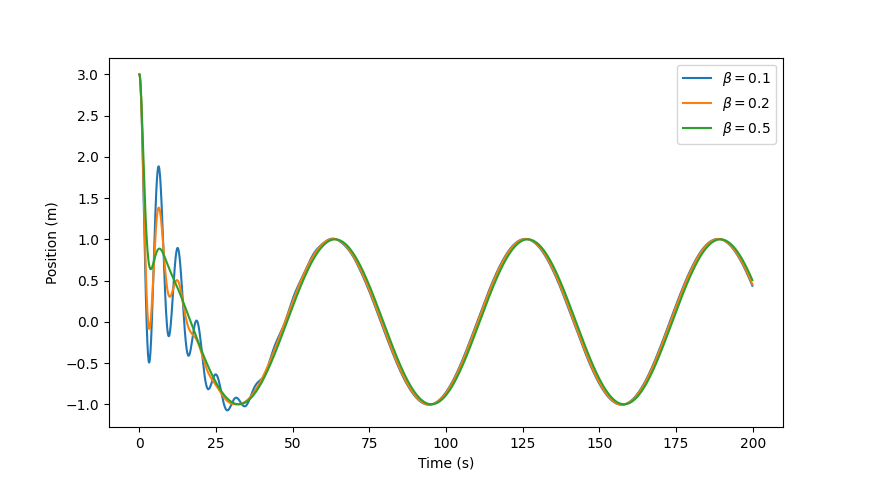
\includegraphics[scale=0.75]{Figure_2.png}
                  \end{center}
                  As is expected here, greater values of $\beta$ result in quicker die-off of the transient solution. $\beta$ only slightly effects
                  the steady-state solution, causing slight displacement as the transient solution never actually reaches zero.

            \item \inputminted[breaklines, autogobble]{python3}{./python/q1/q1f.py}
                  \begin{center}
                        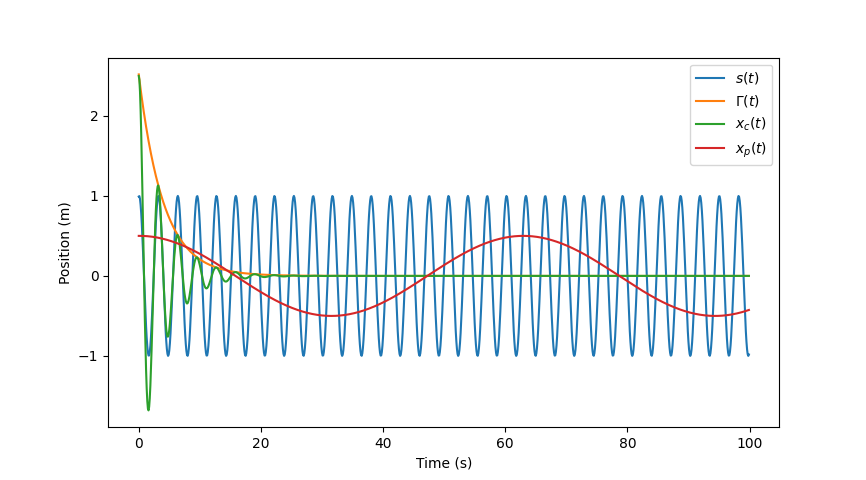
\includegraphics[scale=0.75]{Figure_3.png}
                  \end{center}
                  $s(t)$ contributes the oscillation of the transient solution. $\Gamma(t)$ contributes the exponential decay envelope. $x_c(t)$ contributes,
                  being the product of $s(t)$ and $\Gamma(t)$ produces the initial decaying transient solution. $x_p(t)$ contributes the steady-state solution.

            \item \inputminted[breaklines, autogobble]{python3}{./python/q1/q1g.py}
                  \begin{center}
                        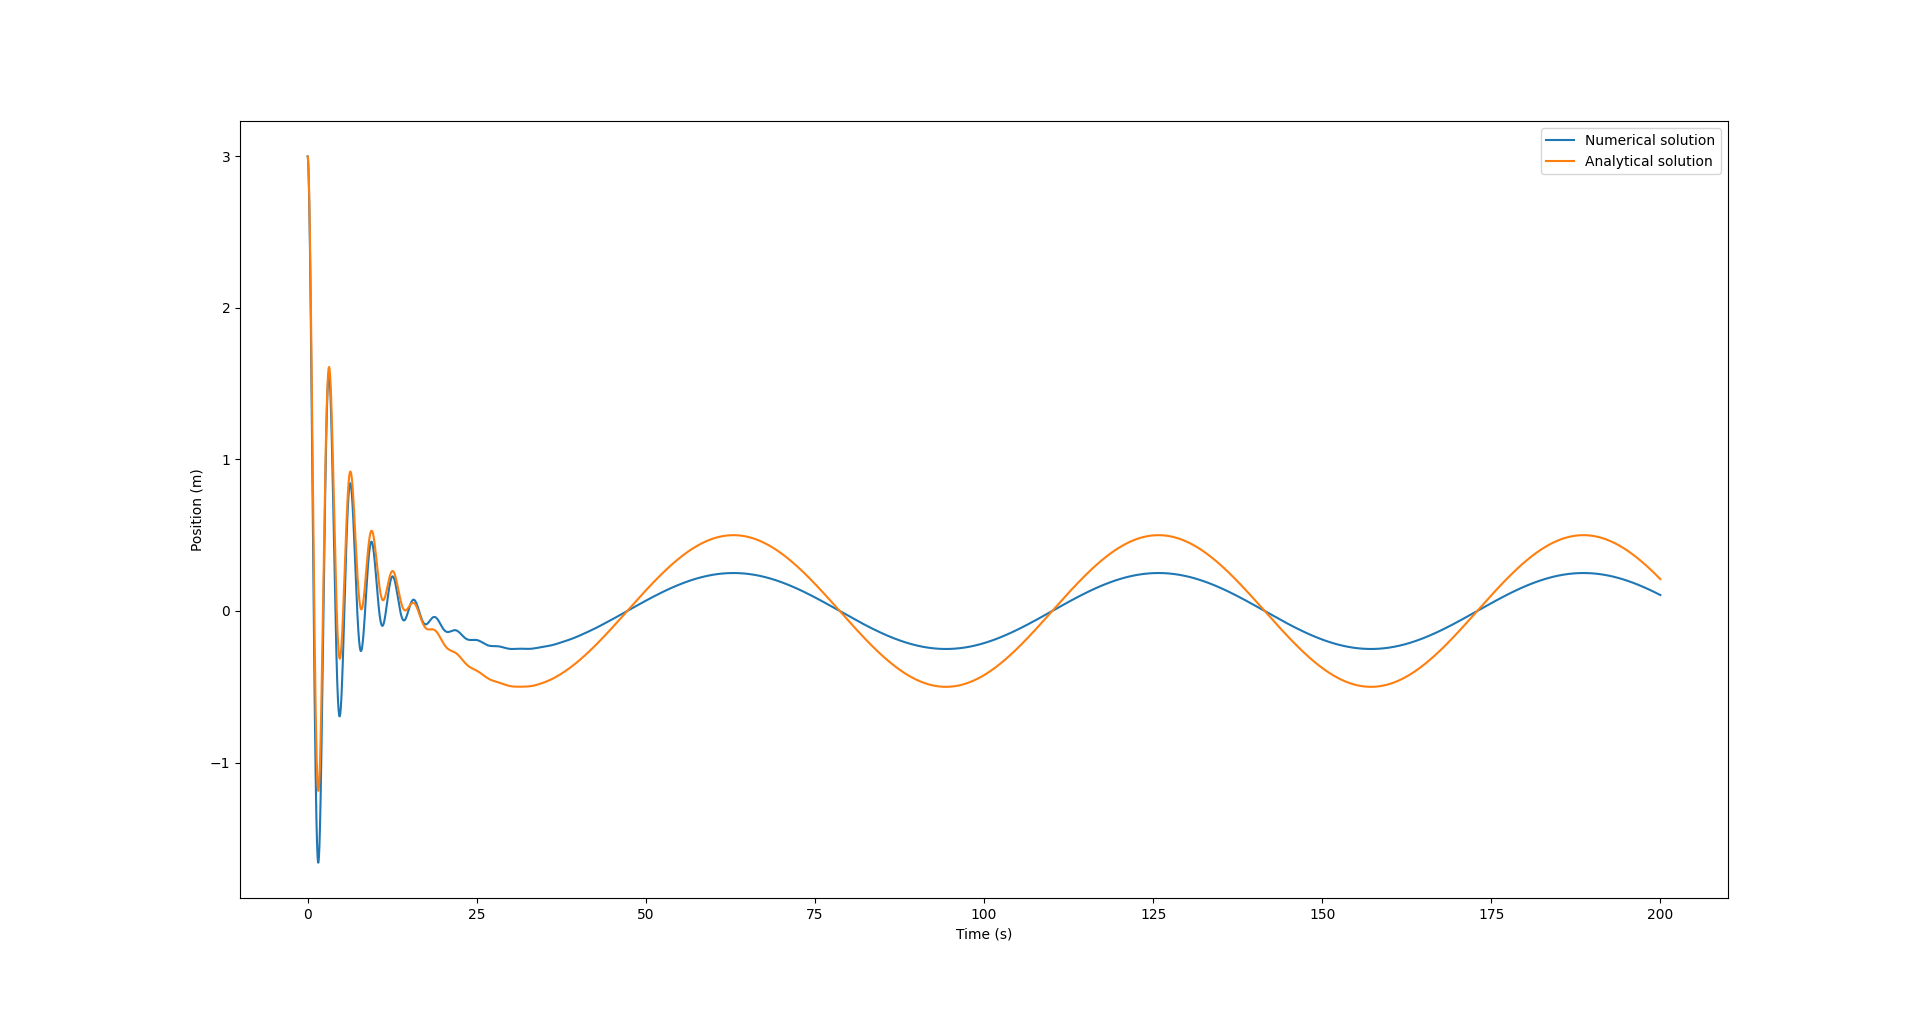
\includegraphics[scale=0.75]{Figure_4.png}
                  \end{center}
      \end{enumerate}
\end{soln}
\newpage

% PROBLEM 2
\begin{problem}
We want to study now the behaviour of the \textbf{non-linear (physical) pendulum}. The analytical solutions we
generally get for oscillating systems are derived under the small-angle approximation, which allows us to write
$\sin(\theta)\approx\theta$. If one drops this hypothesis things change, and the motion now becomes dependent on the amplitude.
The equation of motion is now:
$$\frac{d^2\theta}{dt^2}=-\frac{g}{l}\sin\left(\theta\right)-q\frac{d\theta}{dt}+F_d\sin\left(\Omega_Dt\right)$$
Where the only difference from the linear case is that we now have $\sin\theta$ instead of $\theta$. This equation of motion
has no analytical solutions; therefore, we need to solve it numerically. We thus need to write the equations
for angular acceleration and velocity and use them, e.g., with the Euler-Cromer method:
$$\frac{d\omega}{dt}=-\frac{g}{l}\sin\left(\theta\right)-q\frac{d\theta}{dt}+F_d\sin\left(\Omega_Dt\right)$$
$$\frac{d\theta}{dt}=\omega$$
\begin{enumerate}[label=(\alph*)]
      \item Write a python program that calculates numerically $\theta(t)$ using the Euler-Cromer method.
      \item Write another python program (you can mostly base it on what you wrote in (2a)) that calculates two separate
            solutions $\theta_1(t)$ and $\theta_2(t)$, where $\theta_1(t)$ starts with an initial angle $\theta_0=10\unit{\degree}$ while $\theta_2(t)$ starts with an ever so
            slightly different initial angle $\theta_0=10.05\unit{\degree}$.
      \item In the program you wrote in (2b), add a phase-space plot where you now plot $\omega$ vs. $\theta$.
\end{enumerate}
\end{problem}
\begin{soln}
      \begin{enumerate}[label=(\alph*)]
            \item \inputminted[breaklines, autogobble]{python3}{./python/q2/q2a.py}
                  \begin{center}
                        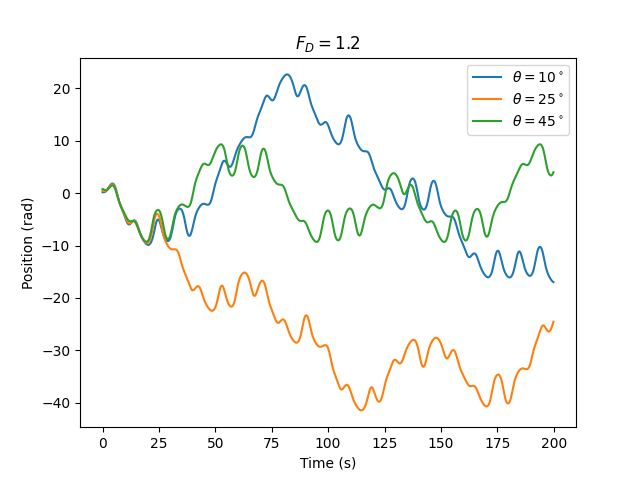
\includegraphics[scale=0.75]{Figure_5-1.png}
                        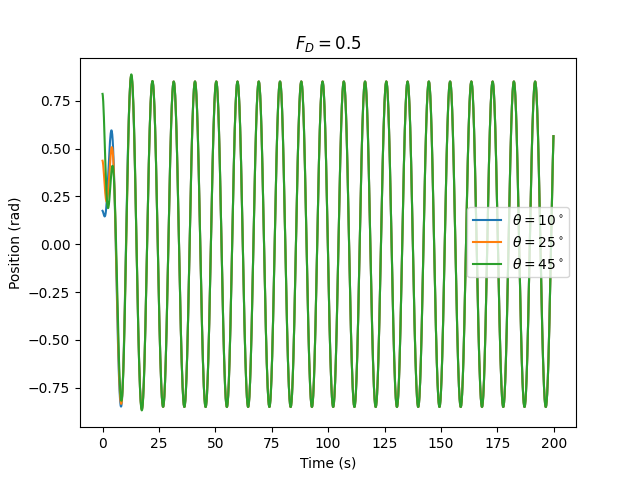
\includegraphics[scale=0.75]{Figure_5-2.png}
                  \end{center}
            \item \inputminted[breaklines, autogobble]{python3}{./python/q2/q2b.py}
                  \begin{center}
                        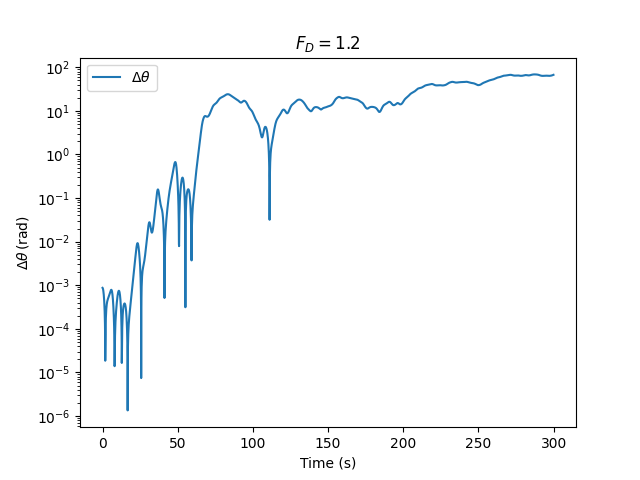
\includegraphics[scale=0.75]{Figure_6-1.png}
                        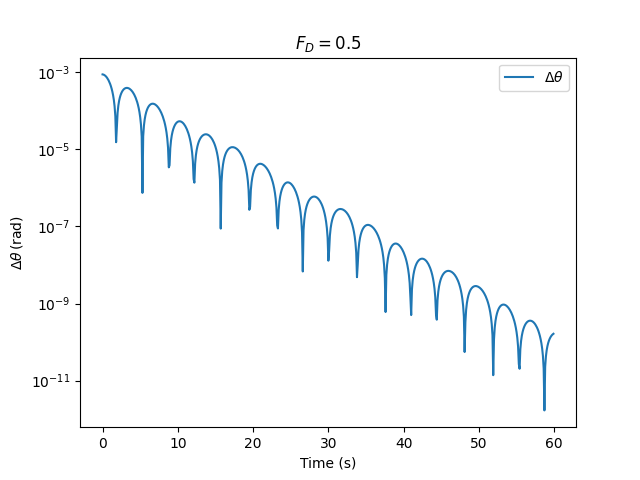
\includegraphics[scale=0.75]{Figure_6-2.png}
                  \end{center}
            \item \inputminted[breaklines, autogobble]{python3}{./python/q2/q2c.py}
                  \begin{center}
                        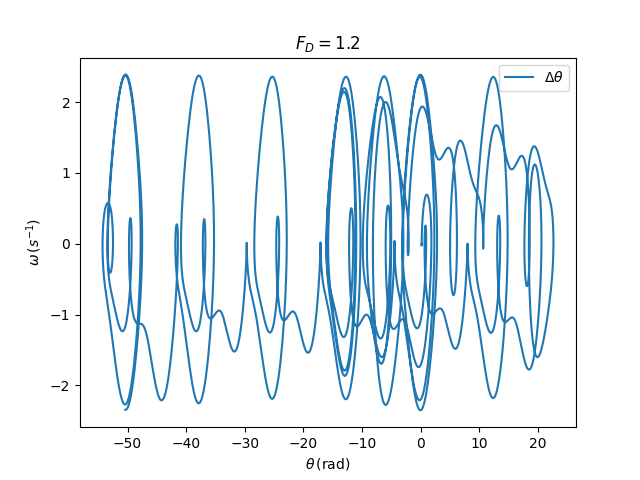
\includegraphics[scale=0.75]{Figure_7-1.png}
                        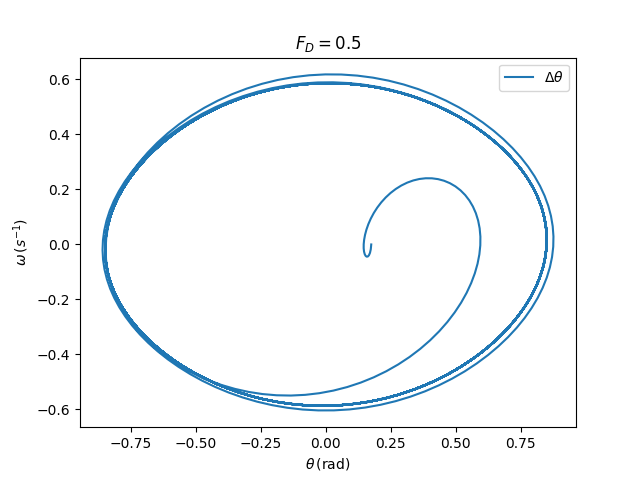
\includegraphics[scale=0.75]{Figure_7-2.png}
                  \end{center}
      \end{enumerate}
\end{soln}
\end{document}